\documentclass[journal,12pt,twocolumn]{IEEEtran}
%
\usepackage{setspace}
\usepackage{gensymb}
%\doublespacing
\singlespacing

%\usepackage{graphicx}
%\usepackage{amssymb}
%\usepackage{relsize}
\usepackage[cmex10]{amsmath}
%\usepackage{amsthm}
%\interdisplaylinepenalty=2500
%\savesymbol{iint}
%\usepackage{txfonts}
%\restoresymbol{TXF}{iint}
%\usepackage{wasysym}
\usepackage{amsthm}
%\usepackage{iithtlc}
\usepackage{mathrsfs}
\usepackage{txfonts}
\usepackage{stfloats}
\usepackage{bm}
\usepackage{cite}
\usepackage{cases}
\usepackage{subfig}
%\usepackage{xtab}
\usepackage{longtable}
\usepackage{multirow}
%\usepackage{algorithm}
%\usepackage{algpseudocode}
\usepackage{enumitem}
\usepackage{mathtools}
\usepackage{steinmetz}
\usepackage{tikz}
\usepackage{circuitikz}
\usepackage{verbatim}
\usepackage{tfrupee}
\usepackage[breaklinks=true]{hyperref}
%\usepackage{stmaryrd}
\usepackage{tkz-euclide} % loads  TikZ and tkz-base
%\usetkzobj{all}
\usetikzlibrary{calc,math}
\usepackage{listings}
    \usepackage{color}                                            %%
    \usepackage{array}                                            %%
    \usepackage{longtable}                                        %%
    \usepackage{calc}                                             %%
    \usepackage{multirow}                                         %%
    \usepackage{hhline}                                           %%
    \usepackage{ifthen}                                           %%
  %optionally (for landscape tables embedded in another document): %%
    \usepackage{lscape}     
\usepackage{multicol}
\usepackage{chngcntr}
%\usepackage{enumerate}

%\usepackage{wasysym}
%\newcounter{MYtempeqncnt}
\DeclareMathOperator*{\Res}{Res}
%\renewcommand{\baselinestretch}{2}
\renewcommand\thesection{\arabic{section}}
\renewcommand\thesubsection{\thesection.\arabic{subsection}}
\renewcommand\thesubsubsection{\thesubsection.\arabic{subsubsection}}

\renewcommand\thesectiondis{\arabic{section}}
\renewcommand\thesubsectiondis{\thesectiondis.\arabic{subsection}}
\renewcommand\thesubsubsectiondis{\thesubsectiondis.\arabic{subsubsection}}

% correct bad hyphenation here
\hyphenation{op-tical net-works semi-conduc-tor}
\def\inputGnumericTable{}                                 %%

\lstset{
%language=C,
frame=single, 
breaklines=true,
columns=fullflexible
}
%\lstset{
%language=tex,
%frame=single, 
%breaklines=true
%}

\begin{document}
%


\newtheorem{theorem}{Theorem}[section]
\newtheorem{problem}{Problem}
\newtheorem{proposition}{Proposition}[section]
\newtheorem{lemma}{Lemma}[section]
\newtheorem{corollary}[theorem]{Corollary}
\newtheorem{example}{Example}[section]
\newtheorem{definition}[problem]{Definition}
%\newtheorem{thm}{Theorem}[section] 
%\newtheorem{defn}[thm]{Definition}
%\newtheorem{algorithm}{Algorithm}[section]
%\newtheorem{cor}{Corollary}
\newcommand{\BEQA}{\begin{eqnarray}}
\newcommand{\EEQA}{\end{eqnarray}}
\newcommand{\define}{\stackrel{\triangle}{=}}
\bibliographystyle{IEEEtran}
%\bibliographystyle{ieeetr}
\providecommand{\mbf}{\mathbf}
\providecommand{\pr}[1]{\ensuremath{\Pr\left(#1\right)}}
\providecommand{\qfunc}[1]{\ensuremath{Q\left(#1\right)}}
\providecommand{\sbrak}[1]{\ensuremath{{}\left[#1\right]}}
\providecommand{\lsbrak}[1]{\ensuremath{{}\left[#1\right.}}
\providecommand{\rsbrak}[1]{\ensuremath{{}\left.#1\right]}}
\providecommand{\brak}[1]{\ensuremath{\left(#1\right)}}
\providecommand{\lbrak}[1]{\ensuremath{\left(#1\right.}}
\providecommand{\rbrak}[1]{\ensuremath{\left.#1\right)}}
\providecommand{\cbrak}[1]{\ensuremath{\left\{#1\right\}}}
\providecommand{\lcbrak}[1]{\ensuremath{\left\{#1\right.}}
\providecommand{\rcbrak}[1]{\ensuremath{\left.#1\right\}}}
\theoremstyle{remark}
\newtheorem{rem}{Remark}
\newcommand{\sgn}{\mathop{\mathrm{sgn}}}
\providecommand{\abs}[1]{\left\vert#1\right\vert}
\providecommand{\res}[1]{\Res\displaylimits_{#1}} 
\providecommand{\norm}[1]{\left\lVert#1\right\rVert}
%\providecommand{\norm}[1]{\lVert#1\rVert}
\providecommand{\mtx}[1]{\mathbf{#1}}
\providecommand{\mean}[1]{E\left[ #1 \right]}
\providecommand{\fourier}{\overset{\mathcal{F}}{ \rightleftharpoons}}
%\providecommand{\hilbert}{\overset{\mathcal{H}}{ \rightleftharpoons}}
\providecommand{\system}{\overset{\mathcal{H}}{ \longleftrightarrow}}
	%\newcommand{\solution}[2]{\textbf{Solution:}{#1}}
\newcommand{\solution}{\noindent \textbf{Solution: }}
\newcommand{\cosec}{\,\text{cosec}\,}
\providecommand{\dec}[2]{\ensuremath{\overset{#1}{\underset{#2}{\gtrless}}}}
\newcommand{\myvec}[1]{\ensuremath{\begin{pmatrix}#1\end{pmatrix}}}
\newcommand{\mydet}[1]{\ensuremath{\begin{vmatrix}#1\end{vmatrix}}}
%\numberwithin{equation}{section}
\numberwithin{equation}{subsection}
%\numberwithin{problem}{section}
%\numberwithin{definition}{section}
\makeatletter
\@addtoreset{figure}{problem}
\makeatother
\let\StandardTheFigure\thefigure
\let\vec\mathbf
%\renewcommand{\thefigure}{\theproblem.\arabic{figure}}
\renewcommand{\thefigure}{\theproblem}
%\setlist[enumerate,1]{before=\renewcommand\theequation{\theenumi.\arabic{equation}}
%\counterwithin{equation}{enumi}
%\renewcommand{\theequation}{\arabic{subsection}.\arabic{equation}}
\def\putbox#1#2#3{\makebox[0in][l]{\makebox[#1][l]{}\raisebox{\baselineskip}[0in][0in]{\raisebox{#2}[0in][0in]{#3}}}}
     \def\rightbox#1{\makebox[0in][r]{#1}}
     \def\centbox#1{\makebox[0in]{#1}}
     \def\topbox#1{\raisebox{-\baselineskip}[0in][0in]{#1}}
     \def\midbox#1{\raisebox{-0.5\baselineskip}[0in][0in]{#1}}
\vspace{3cm}
\title{Forming a Correlation Matrix}
\author{C ANISH}
%\title{
%	\logo{Matrix Analysis through Octave}{\begin{center}\includegraphics[scale=.24]{tlc}\end{center}}{}{HAMDSP}
%}
% paper title
% can use linebreaks \\ within to get better formatting as desired
%\title{Matrix Analysis through Octave}
%
%
% author names and IEEE memberships
% note positions of commas and nonbreaking spaces ( ~ ) LaTeX will not break
% a structure at a ~ so this keeps an author's name from being broken across
% two lines.
% use \thanks{} to gain access to the first footnote area
% a separate \thanks must be used for each paragraph as LaTeX2e's \thanks
% was not built to handle multiple paragraphs
%
%\author{<-this % stops a space
%\thanks{}}
%}
% note the % following the last \IEEEmembership and also \thanks - 
% these prevent an unwanted space from occurring between the last author name
% and the end of the author line. i.e., if you had this:
% 
% \author{....lastname \thanks{...} \thanks{...} }
%                     ^------------^------------^----Do not want these spaces!
%
% a space would be appended to the last name and could cause every name on that
% line to be shifted left slightly. This is one of those "LaTeX things". For
% instance, "\textbf{A} \textbf{B}" will typeset as "A B" not "AB". To get
% "AB" then you have to do: "\textbf{A}\textbf{B}"
% \thanks is no different in this regard, so shield the last } of each \thanks
% that ends a line with a % and do not let a space in before the next \thanks.
% Spaces after \IEEEmembership other than the last one are OK (and needed) as
% you are supposed to have spaces between the names. For what it is worth,
% this is a minor point as most people would not even notice if the said evil
% space somehow managed to creep in.
% The paper headers
%\markboth{Journal of \LaTeX\ Class Files,~Vol.~6, No.~1, January~2007}%
%{Shell \MakeLowercase{\textit{et al.}}: Bare Demo of IEEEtran.cls for Journals}
% The only time the second header will appear is for the odd numbered pages
% after the title page when using the twoside option.
% 
% *** Note that you probably will NOT want to include the author's ***
% *** name in the headers of peer review papers.                   ***
% You can use \ifCLASSOPTIONpeerreview for conditional compilation here if
% you desire.
% If you want to put a publisher's ID mark on the page you can do it like
% this:
%\IEEEpubid{0000--0000/00\$00.00~\copyright~2007 IEEE}
% Remember, if you use this you must call \IEEEpubidadjcol in the second
% column for its text to clear the IEEEpubid mark.
% make the title area
\maketitle
\newpage
%\tableofcontents
\bigskip
\renewcommand{\thefigure}{\theenumi}
\renewcommand{\thetable}{\theenumi}
%\renewcommand{\theequation}{\theenumi}
%\begin{abstract}
%%\boldmath
%In this letter, an algorithm for evaluating the exact analytical bit error rate  (BER)  for the piecewise linear (PL) combiner for  multiple relays is presented. Previous results were available only for upto three relays. The algorithm is unique in the sense that  the actual mathematical expressions, that are prohibitively large, need not be explicitly obtained. The diversity gain due to multiple relays is shown through plots of the analytical BER, well supported by simulations. 
%
%\end{abstract}
% IEEEtran.cls defaults to using nonbold math in the Abstract.
% This preserves the distinction between vectors and scalars. However,
% if the journal you are submitting to favors bold math in the abstract,
% then you can use LaTeX's standard command \boldmath at the very start
% of the abstract to achieve this. Many IEEE journals frown on math
% in the abstract anyway.
% Note that keywords are not normally used for peerreview papers.
%\begin{IEEEkeywords}
%Cooperative diversity, decode and forward, piecewise linear
%\end{IEEEkeywords}
% For peer review papers, you can put extra information on the cover
% page as needed:
% \ifCLASSOPTIONpeerreview
% \begin{center} \bfseries EDICS Category: 3-BBND \end{center}
% \fi
%
% For peerreview papers, this IEEEtran command inserts a page break and
% creates the second title. It will be ignored for other modes.
%\IEEEpeerreviewmaketitle
\begin{abstract}
This is a document explaining a method to find the Correlation Matrix.
\end{abstract}
Download all python codes from 
%
\begin{lstlisting}
svn co https://github.com/chakki1234/Winter_intern/tree/main/correlation_matrix/codes
\end{lstlisting}

A video explaining the process documented can be found through the link
\begin{lstlisting}
https://drive.google.com/file/d/1GKquFbnmw6De4ltrgvEE7SbDHoYYe6nG/view?usp=sharing
\end{lstlisting}

\section{Solution}
\renewcommand{\theequation}{\theenumi}
\begin{enumerate}[label=\thesection.\arabic*.,ref=\thesection.\theenumi]
\numberwithin{equation}{enumi}

\item $aigiri.txt$ contains a stothram in Telugu. The stothram is split into two files $aigiri\_test1.txt$ and $aigiri\_test2.txt$. The three files are read and each telugu character in the file is converted to its unicode value and is written onto $unicode.txt$, $unicode\_test1.txt$ and $unicode\_test2.txt$ respectively.
\begin{lstlisting}[language=Python]
def read(file_name):
  sloka = open(file_name, 'r')
  sloka_txt = sloka.read()
  sloka.close()
  return sloka_txt
\end{lstlisting}

\begin{lstlisting}[language=Python]
def split_to_words(txt, out_file_name):
  words = txt.split()
  uni_file = open(out_file_name, 'w')

  for i in words:
      if(i !='|' and i !='||' and not(i.isdigit())):
          for j in i:
              uni_file.write('U+' + hex(ord(j)).replace('x', ''))
              uni_file.write('  ')

  uni_file.close()
  
split_to_words(read('aigiri_test1.txt'), 'unicode_test1.txt')
split_to_words(read('aigiri_test2.txt'), 'unicode_test2.txt')
split_to_words(read('aigiri.txt'), 'unicode.txt')
\end{lstlisting}

\item $unicode.txt,\  unicode\_test1.txt$ and $unicode\_test2.txt$ are read and are split into a list of individual unicode values with the help of the function $read\_and\_split$. $uni\_chars\_list$ is a list which contains the list of unicode values from $unicode\_test1.txt$ and $unicode\_test2.txt$.
\begin{lstlisting}[language=Python]
uni_chars_list = []
aigiri_chars = read_and_split('unicode.txt')
uni_chars_list.append(read_and_split('unicode_test1.txt'))
uni_chars_list.append(read_and_split('unicode_test2.txt'))
\end{lstlisting}

\item A for loop runs through the list $uni\_chars\_list$. In the first iteration the variable $uni\_chars$ is the list of all the unicode values from the file $unicode\_test1.txt$. Each individual unicode value from the file is taken and its periodicity is found through the function $to\_cal\_periodicity$.
All the unicode values whose periodicity is found is appended to the list $periodicity\_found$. A dictonary called $periodicity$ is created and a key with the name of the unicode value whose periodicity has to been found is added to the dictonary and its value is initialized to an empty list.  
\begin{lstlisting}[language=Python]
for file_no, uni_chars in enumerate(uni_chars_list):
  global periodicity_found 
  global periodicity 
  global processed_periodic_dict 
  global test_results

  if file_no != 0:
    periodicity_found = []
    periodicity = {}
    processed_periodic_dict = {}

  for i, char in enumerate(uni_chars):
    if char in periodicity_found:
      pass
    else:
      periodicity_found.append(char)
      periodicity[char] = []
      to_cal_periodicity(char, i, file_no)
    
  print(periodicity)
  to_process_dict(periodicity)
  print(processed_periodic_dict)
  plot_bar(processed_periodic_dict)
  test_results.append(processed_periodic_dict)
\end{lstlisting}

\item The function $to\_cal\_periodicity$ calculates the periodicity of an unicode value which is passed as an argument. The function also takes in the index of the unicode value and the file number. The function scans all the unicode values in the file from the index and calculates the number of unicode values in between two consequitive occurences of the unicode value passed as an argument. This count is appended to the empty list declared using the previous code.
\begin{lstlisting}[language=Python]
def to_cal_periodicity(char, index, file_no):
    count = 0
    temp = uni_chars_list[file_no][index+1:]
    for j in temp:
        if j == char:
            periodicity[char].append(count)
            count = 0
        else:
            count = count + 1
\end{lstlisting}

\item After excuting the previous function the dictonary $periodicity$ contains all the unique unicode value as its key and each key has a corresponding periodicity list. The function 
$to\_process\_dict$ takes the dictonary $periodicity$ as its argument. It converts all the keys which are presently unicode values to telugu characters and finds the average of the elements in the corresponding list and normalizes the value with the total number of unicode values in the stothram.  
\begin{lstlisting}[language=Python]
def to_process_dict(periodicity_dict):
    dict_keys = periodicity_dict.keys()
    
    for key in dict_keys:
        if len(periodicity_dict[key]) == 0:
            average = 0
        else:
            average = sum(periodicity_dict[key])/len(periodicity_dict[key])
        key = key.replace('U+', '')
        key = key[:1] + 'x' + key[1:]
        processed_periodic_dict[chr(int(key, 16))] = average/len(aigiri_chars)
\end{lstlisting}

\item The function $plot\_bar$ plots the key value pairs of the dictonary $processed\_periodic\_dict$.
\begin{lstlisting}[language=Python]
def plot_bar(periodicity_dict):
    values = list(periodicity_dict.values())
    keys = [ hex(ord(i)).replace('x', '') for i in list(periodicity_dict.keys()) ]

    fig = plt.figure()
    ax = fig.add_axes([0, 0, 5, 5])
    ax.bar(keys, values)
    plt.show()
\end{lstlisting}

\item The same process is repeated for the list of unicode values in the file $unicode\_test2.txt$. The final $processed\_periodic\_dict$ obtained after iterating through each file is appended to the variable $test\_results$.

\item The variable $test\_results$ is a list which contians the processed dictonary of both the files. The common keys between these two dictonaries is found and is appended to the list $common\_keys$ 
\begin{lstlisting}[language=Python]
common_keys = []
test1_result, test2_result = test_results

for i in  list(test1_result.keys()):
  if i in list(test2_result.keys()):
    common_keys.append(i)
\end{lstlisting}

\item Two new dictonaries are $key\_value\_1$ and $key\_value\_2$ are created. $key\_value\_1$ contains keys form the list $common\_keys$ and the corresponding value which is obtained from the processed dictonary of file 1.  $key\_value\_2$ contains keys form the list $common\_keys$ and the corresponding value which is obtained from the processed dictonary of file 2. The key value pairs of both these dictonaries are plotted to see if the pattern found from $aigiri\_test1.txt$ is also present in $aigiri\_test2.txt$.
\begin{lstlisting}[language=Python]
x_pos = np.linspace(0, 9, 41)
barWidth = 0.05
fig = plt.subplots(figsize =(20, 20)) 
common_keys = [ ord(i) for i in common_keys ]

plt.bar(x_pos, list(key_value_1.values()), color ='r', width = barWidth, 
		edgecolor ='grey', label ='aigiri_test1') 
plt.bar(x_pos + barWidth, list(key_value_2.values()), color ='g', width = barWidth, 
		edgecolor ='grey', label ='aigiri_test2') 

plt.xticks(x_pos, common_keys)
plt.legend()
plt.savefig('normalized.png')
plt.savefig('normalized.eps')
plt.show() 
\end{lstlisting}

\newpage
\item The result obtained is \textbf{\ref{fig:bar}}. It can be observed that the periodicity of most characters obtained from $aigiri\_test1.txt$ follows the same pattern in the remaining verses of the stothram. 
\begin{figure}[!t]
\centering
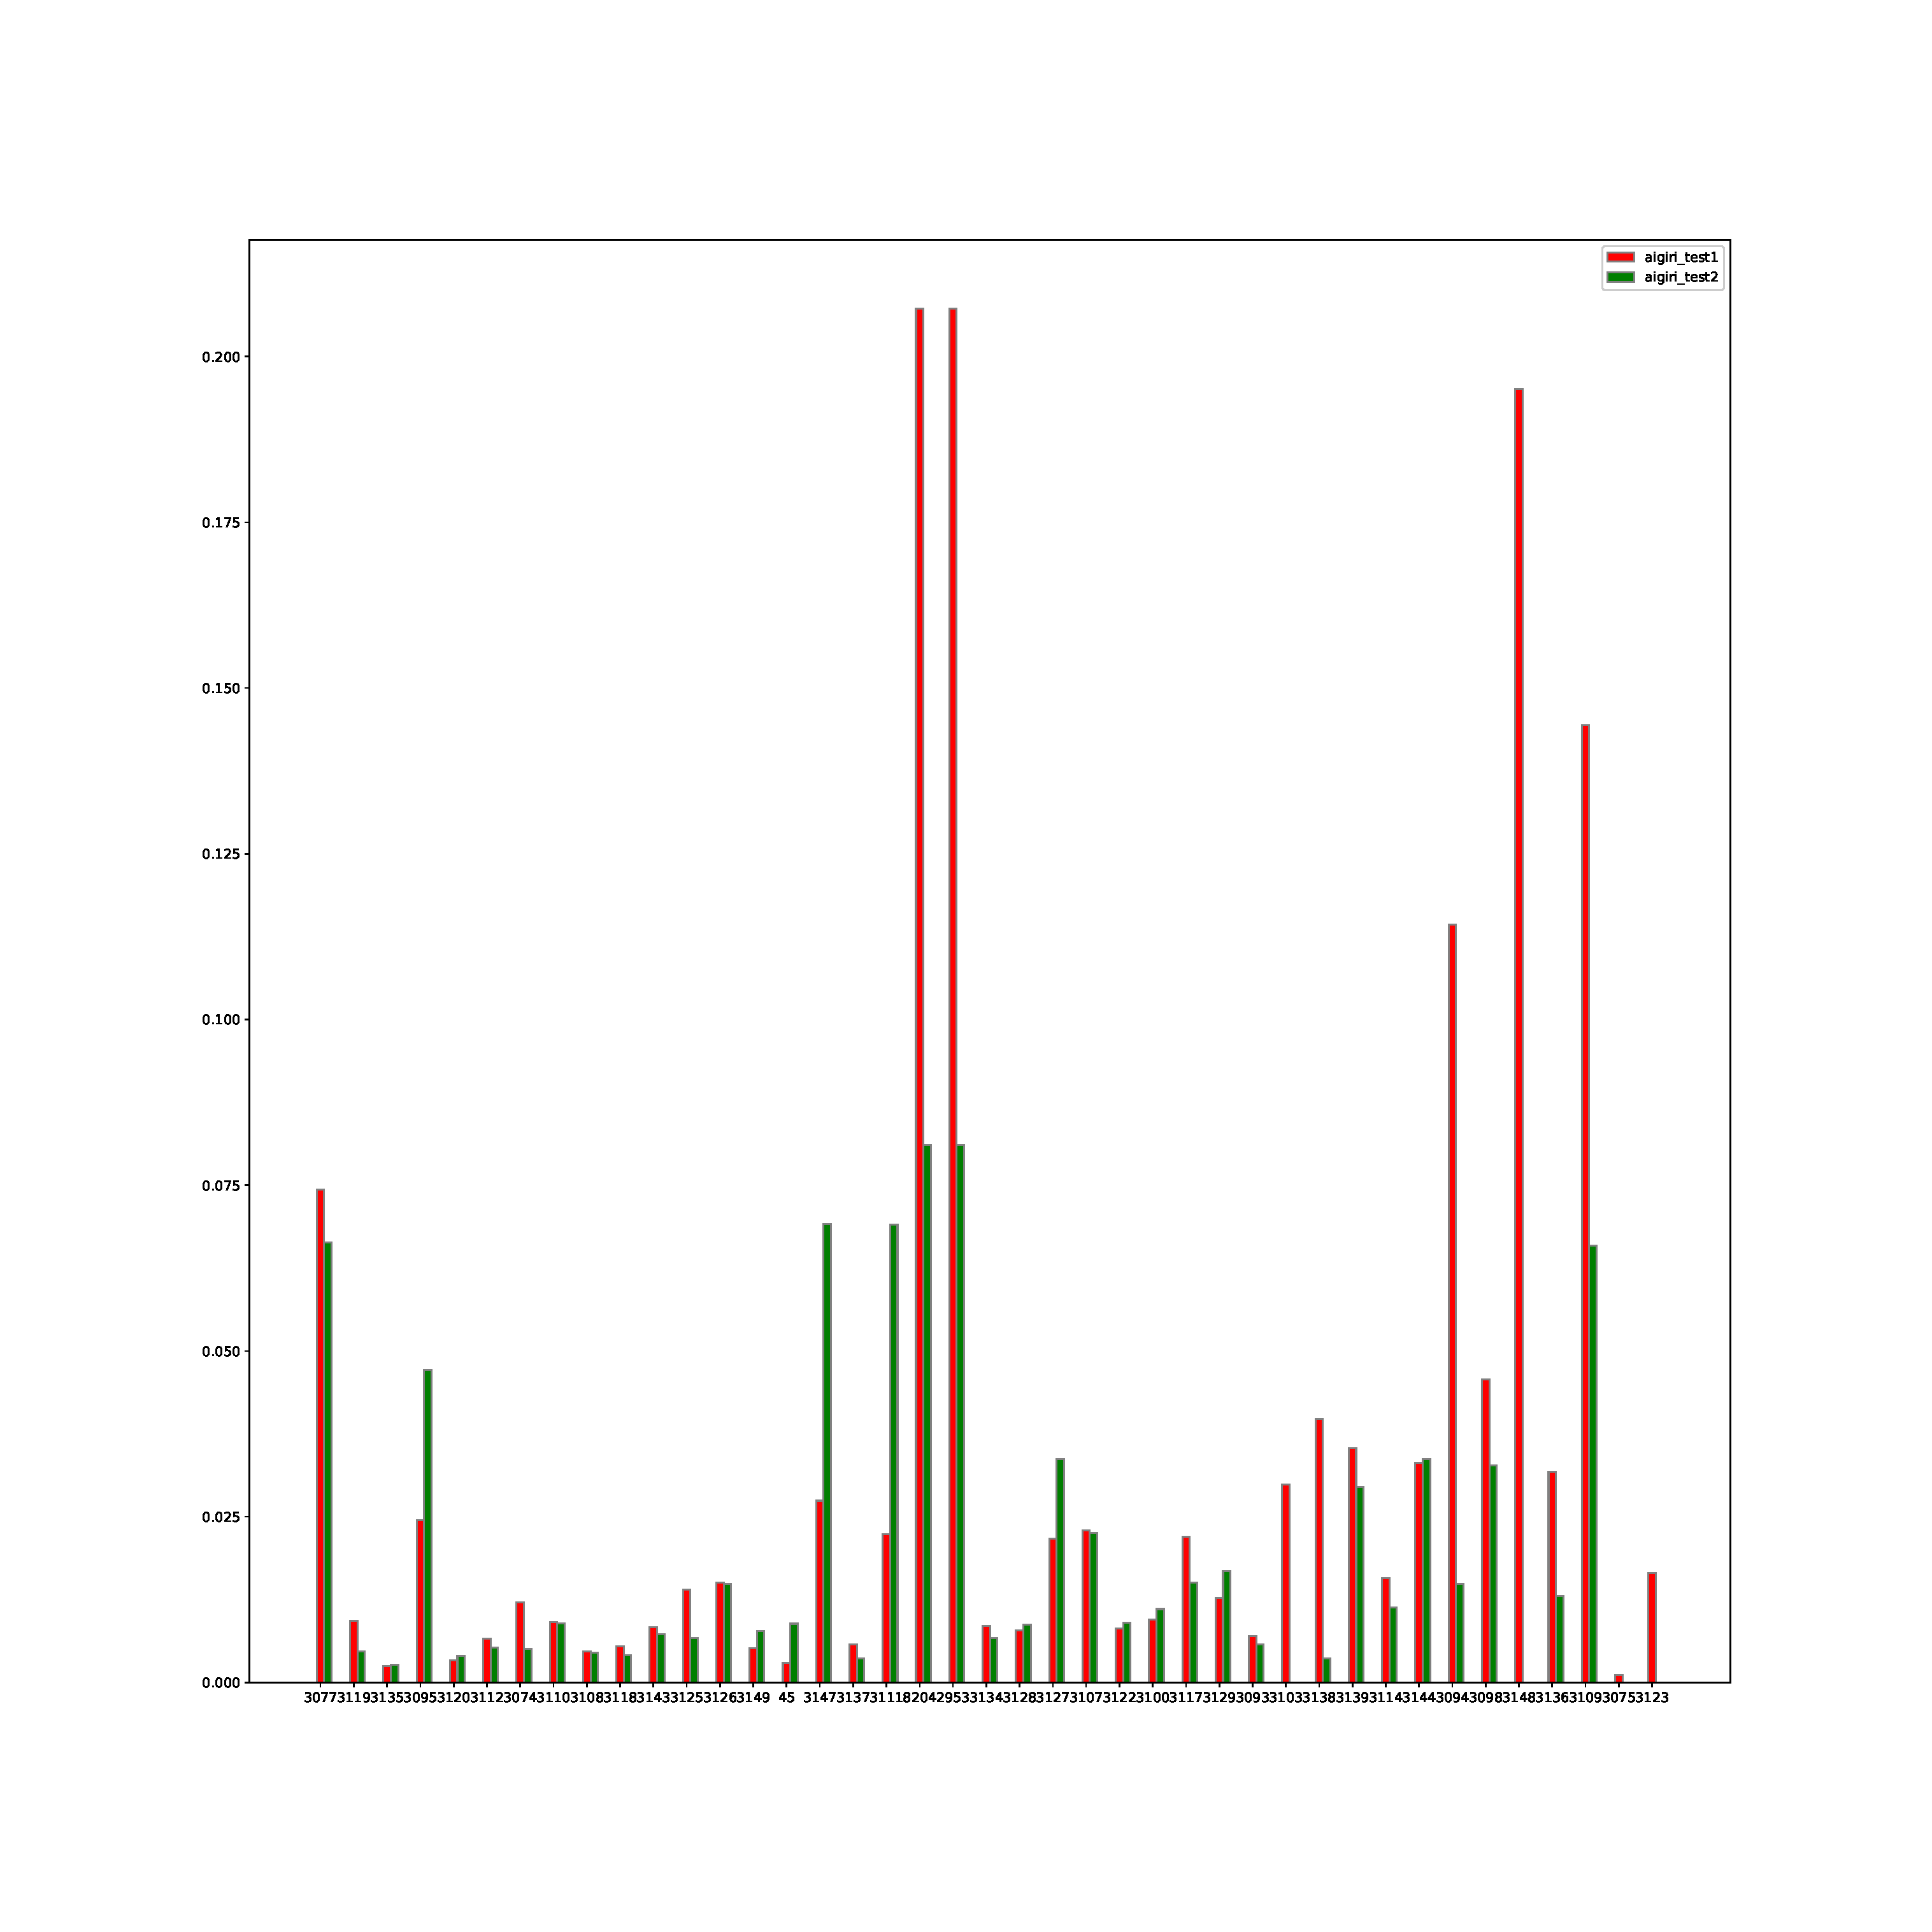
\includegraphics[width=\columnwidth]{./figs/normalized.eps}
\caption{Bar graph depicitng the periodicity of the common characters}
\label{fig:bar}
\end{figure} 

\end{enumerate}


\end{document}
